\chapter{The Simons Observatory: Characterizing the Small Aperture Telescope with Radio Holography}
\label{ch:sat_holo}
This chapter presents holography measurements of the Simons Observatory Small Aperture Telescope at the University of California, San Diego, and preliminary characterization of its optical performance.  This work was made possible by the collaboration of Tommy Alford, Kathleen Harrington and Jeff McMahon from the University of Chicago, Remington Gerras from the University of Southern California, and Joe Seibert, Tran, Tsan, JB LLoyd, Michael Randall, and Kam Arnold from the University of California, San Diego.

\section{Introduction}
The Simons Observatory (SO) will employ three Small Aperture Telescopes (SATs) to measure the largest angular scales visible from the Atacama Desert in Chile.  One SAT has an aperture diameter of 0.42\,m and will measure roughly 10\% of the sky with more than 300,000 bolometer detectors across the three SATs~\cite{2020SPIE11445E7LK}.  Among the three SAT's are three frequency bands -- each with 10,000 detectors: Low-Frequency (LF) bands are centered at 27 and 39\,GHz, Mid-Frequency (MF) bands are centered at 93 and 145\,GHz, and Ultra-High-Frequency (UHF) bands are centered at 225 and 280\,GHz

Mapping the three frequency bands will allow for the separation of the CMB from galactic foregrounds (sourced from synchrotron and dust radiation).  The primary goal of the SATs is to measure the primordial tensor-to-scalar ratio, $r$, to within $\sigma(r) = 0.003$, which is one of SO's many ambitious science goals~\cite{ali20}.  Another ambitious science goal is to characterize the tiny polarization signal of the CMB.  Primordial B-mode spectra peaks at $\ell\approx90$ (or roughly $2^{\circ}$), and therefore precision measurements at large angular scales are critical.

We present the laboratory testing of the MF Small Aperture Telescope using the technique of near-field radio holography.  ``Holography" refers to the measurement of the complex monochromatic electric field wavefront using the interference between a modulated and reference signal.  Radio holography takes advantage of the antenna theory relationship: the far-field radiation pattern of a reflector antenna is the Fourier Transformation of the field distribution in the aperture plane of the antenna~\cite{alma_holog}.

\begin{figure*}[t!]
    \centering
    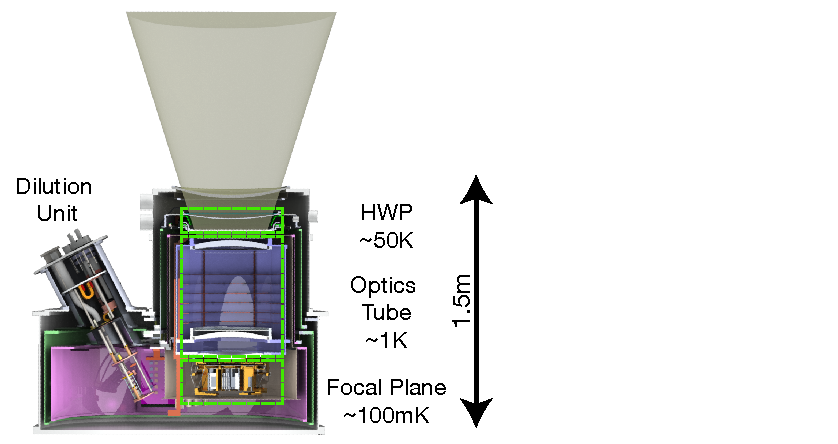
\includegraphics[width = \textwidth]{Figures/sat_optics.pdf}
    \caption{Left: Cross-section of the Small Aperture Telescope (SAT) optics tube.  Light enters through the high-density polyethylene window (UHMWPE) and through the cryogenic half-wave plate (CHWP).  The lenses re-image the beam onto the focal plane, where the holography detector measures power and phase at a given source position.  Right: SAT cryostat used in holography testing (Photo credit: Remington Gerras).}
    \label{fig:sat_optics}
\end{figure*}

Near-field holography of the SAT maps the wavefront emerging from the cryostat.  Using Fresnel diffraction (FD)~\cite{Goodman2005-ne}, these measured fields can be propagated to determine the far-field beam pattern of the telescope fed by this feedhorn receiver.  Moreover, these beams are useful for the identification and mitigation of optical problems within the receiver (i.e. optical aberrations, focus, scattered power, etc.).  These measurements enable a detailed verification of system-level optical performance prior to the deployment of a receiver on a telescope.

In Section~\ref{sec:sat_optics_tube} we describe the optical design and components of the SO SAT optics tube.  In Section~\ref{sec:satot_meas_method} we describe the measurement approach including the cryogenic receiver (\ref{sec:sat_cryo_rec}) and holography hardware (\ref{sec:sat_meas_hardware}) required for measuring beam maps (full details can be found in Appendix~\ref{sec:appendix_hardware}).  In Section~\ref{sec:sat_results} we present the measured beam maps.   Section~\ref{sec:sat_prop_fields} discusses analysis methods to propagate the measured beams into the far-field using FD.  We conclude with a discussion of future applications of this approach in Section~\ref{sec:sat_discussion}.  
\section{SO Small Aperture Telescope Optics Tubes Design}
\label{sec:sat_optics_tube}

\begin{figure}[t!]
    \centering
    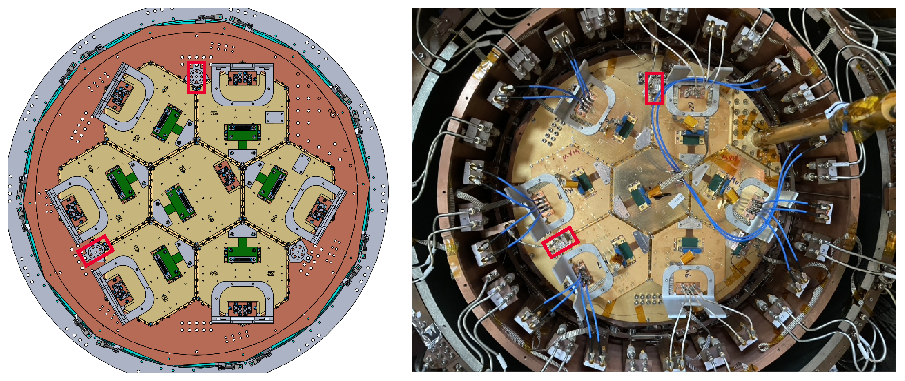
\includegraphics[width = \textwidth]{Figures/sat_fpa.pdf}
    \caption{SAT Focal Plane.  The two holography receivers are outlined in red, separated by $120^{\circ}$.  Two receivers are installed for redundancy, but also served as a useful tool when characterizing systematics (such as ``ghosting", or spurious signal in the beam maps, and polarization effects).}
    \label{fig:sat_fpa}
\end{figure}

Here we provide a brief overview of the SAT optics, starting at the window of the telescope and ending at the detectors.  The full SAT design is described in~\cite{ali20,2020SPIE11445E7LK} and shown in Figure~\ref{fig:sat_optics}.


Light enters through a 3\,mm thick ultra-high molecular weight polyethylene hexagonal window with an anti-reflection coating~\cite{zhu18}.  A Cryogenic Half-Wave Plate (CHWP) polarization modulator then reconstructs the polarization of the CMB at 40\,K.  For the duration of these holography measurements, the CHWP is held at a fixed angular orientation.  A 1\,K Lyot stop is the first cold optical element, and is followed by the SAT refractor.

The SAT optics is purely refractive; three anti-reflection coated silicon lenses~\cite{Datta:13,golec20} control the beam size and shape onto seven hexagonal detector arrays.  The SAT lenses are the largest Si lenses used for a CMB telescope to date~\cite{ali20}.  Baffles line in the inside of the SAT refractor to control spurious scattering.  Photons are then coupled onto the detectors by individual feedhorns. Seven hexagonal detector arrays are housed in the focal plane of the optics tube at 100\,mK.

\section{Measurement Approach}
\label{sec:satot_meas_method}
Here, we describe the hardware in two sections: 1) a cryogenic optics tube and 2) the holography system comprised of a source, correlation receiver, and motion system.
\subsection{Cryogenic System}
\label{sec:sat_cryo_rec}
The optics tube is housed in the SAT cryostat\cite{2020SPIE11445E7LK}.  The cryostat holds and cools the optics tube and provides support for detector readout.  This setup supports up to seven detector arrays (Fig.~\ref{fig:sat_fpa}).   In the test configuration, all bolometric arrays~\cite{2022arXiv220104507H} are filled in the focal plane, and two holography feedhorns are added to the edges of the focal plane, each separated by $120^{\circ}$.

The holography detectors consist of a feedhorn  identical to that used for the bolometric detectors, but with standard wave guide flanges at the outputs. A receiver consisting of a round to rectangular wave guide transition and a harmonic mixer is attached to this feed array.  The mixer was designed to operate from 70-110\,GHz, but was found to operate satisfactorily up to 170\,GHz. For operational simplicity, we used this mixer over our full frequency range from 85-135\,GHz.

Two identical receivers are installed in the focal plane for redundancy.  Two 0-18\,GHz coaxial connections were made from the receiver to connectors at the cryostat wall.  These coaxes are heat sunk at various stages between the focal plane, which was operated at 4\,K while doing holography, and the 300\,K cryostat wall.  A separate cool down was used to measure the loss along these coaxial feed lines.  The loss  was found to be 23\,dB at the LO frequency (10-13\,GHz).  Accurate knowledge of the loss along the feed lines is critical for providing the correct amount of power to the mixers in the focal plane.  The loss at the interference frequencies (IF) (100\,MHz) is significantly lower and not critical to the function of this system.

\begin{figure}[t!]
    \centering
    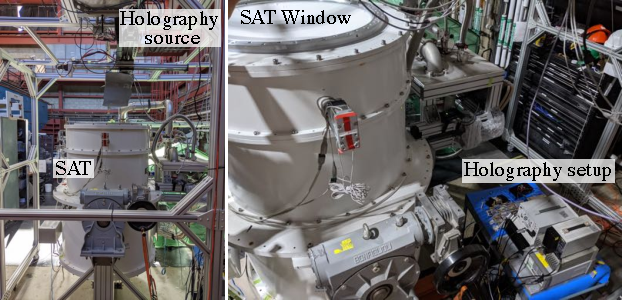
\includegraphics[width = \textwidth]{Figures/sat_exp.pdf}
    \caption{Lab photos of the holography setup on the SAT.  Left: The holography source, covered in a sheet of eccosorb to control scattering, is centered above the SAT window and points directly into the SAT, sitting below.  Right: The holography electronics sit on a cart next to the SAT readout.  The SAT window in the top left is made of UHMWPE.}
    \label{fig:sat_hardware}
\end{figure}

\subsection{Holography System}
\label{sec:sat_meas_hardware}

Figure~\ref{fig:setup} shows a schematic overview of the holography hardware.  Two millimeter-wave sources are used to measure the full SO MF band: F90 (80-120\,GHz) and F150 (130-170\,GHz).  Only one source is mounted at a given time.  The source is broadcast into the receiver using standard gain feed horns held close to the window ($\approx10$\,cm) (Figure~\ref{fig:sat_hardware}).

A motorized two-dimensional stage holds the source and is mounted on a support structure above the SAT.  During a measurement, the source (frequency is fixed) is moved over a $80\times80$\,cm range with 1\,cm steps.  One map takes roughly 2 hours to complete.

A common local oscillator (LO2 in Figure~\ref{fig:setup}) is fed to two harmonic mixers: 1) picked off from the source and 2) at the output of the cryogenic receiver.  The IF signal from both mixers in the 0-100\,MHz band is amplified and passed to a digital correlator (Casper ROACH2 ~\cite{roach2}) which computes the complex correlation between the two signals~\cite{ches18}.  The FPGA on the ROACH2 board outputs the amplitude and the phase of the correlated output, subdivided into a number of 100\,kHz wide bins.  Only the bin associated with the IF frequency is used in subsequent analysis.  The software to program and analyze output from the FPGA is made public on the \textit{McMahonCosmologyGroup} GitHub page in a package called \verb|holog-exp|~\cite{holog-exp}.  Appendix~\ref{app:holog} provides further details on the hardware of the holography setup.

Due to the presence of the CHWP, the source's polarized signal is modulated upon entering the optics tube.  Therefore, to understand the effects of the CHWP, we measure two beam maps at each frequency: with a waveguide twist at the output of the source, and without a waveguide twist.  This allows us to measure the response of the optics tube at two source polarizations (the waveguide twist changes the source polarization by $90^{\circ}$).

 \begin{figure}[t!]
    \centering
    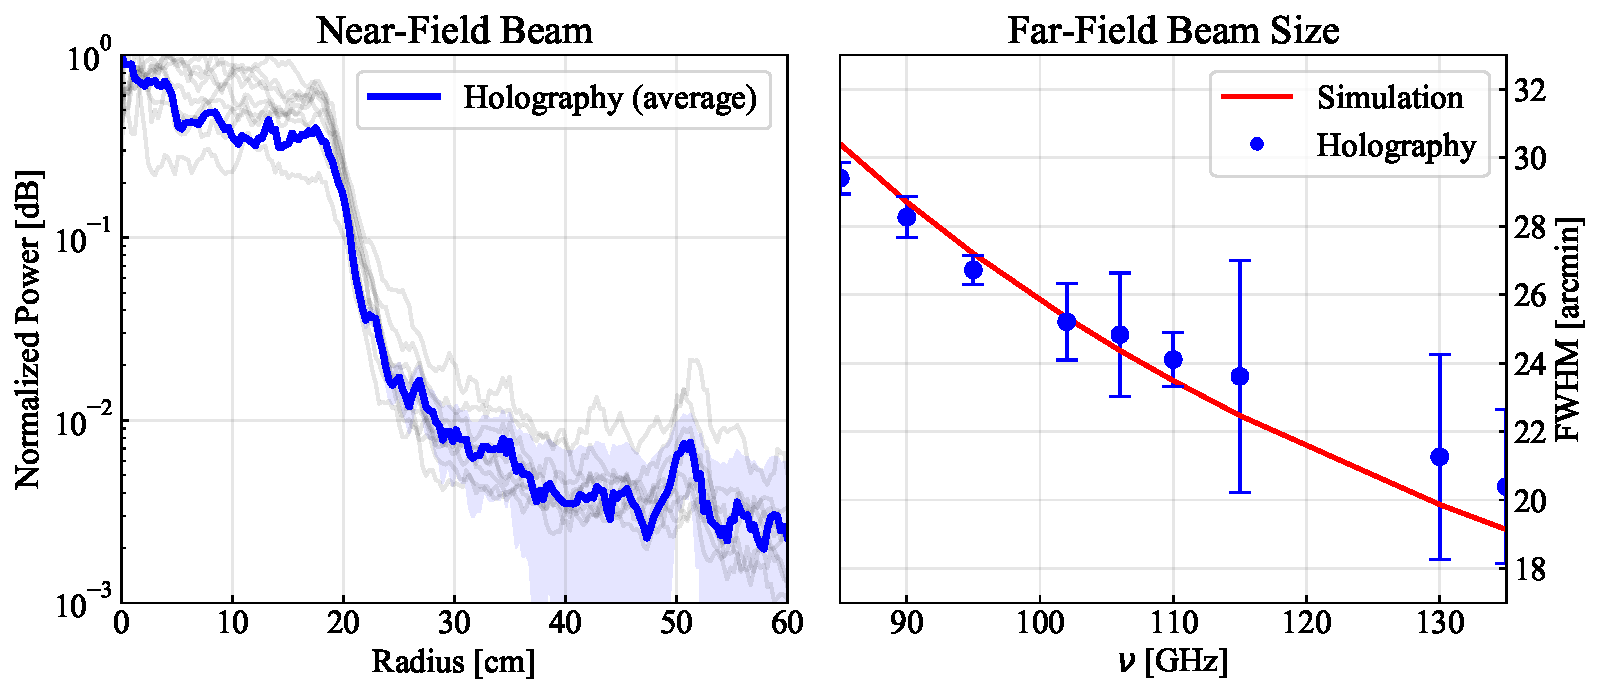
\includegraphics[width =\textwidth]{Figures/SAT_MF1_beam.pdf}
    \caption{Left: Preliminary near-field beam shape of the SAT in MF-1.  Beams are averaged over all frequencies measured, and the averaged beam is then radially averaged to get the near-field beam profile.  Right: Preliminary beam sizes of the SO SAT in MF-1.  Far-field beams measured with holography (blue) are radially binned and the FWHM is obtained from the resulting 1D beam profile.  Simulations are obtained using a diffractive optics simulation, and plotted are where the measured beam sizes with $2\sigma$ errorbars.}
    \label{fig:sat_fwhm}
\end{figure}

\section{Results and Interpretation}
\label{sec:sat_results}

\subsection{Near-Field Beam Maps}
Figure~\ref{fig:sat_mf_cobeam} and ~\ref{fig:sat_mf_crbeam} show the measured power and phase of the beam maps, respectively, at each frequency.   A variable attenuator at the output of the source was used to optimize the amount of signal entering the optics tube, to ensure power was not too high such that the measurement was saturated, but to also ensure the signal was high enough for signal-to-noise greater than 35\,dB.

Each beam map is labeled either $0^{\circ}$ WG, with a straight waveguide at the source output, or $90^{\circ}$ WG, with a waveguide twist at the source output.  These labels also correspond to the $E_x$ and $E_y$ fields.  We assume the source and receiver to be misaligned; to account for this, we rotate the two beams by $\theta$ which is fit to minimize $E_y^{'}$:

\begin{equation}
\begin{bmatrix}
 E_x^{'} \\
 E_y^{'}
 \end{bmatrix} = 
\begin{bmatrix}
 \cos(\theta) & \sin(\theta) \\
 -\sin(\theta) & \cos(\theta)
 \end{bmatrix}
\begin{bmatrix}
 E_x \\
 E_y
 \end{bmatrix}
 \end{equation}
 
The shape of the main beam was found to be in good agreement with simulations at all frequencies (Figure~\ref{fig:sat_fwhm}).  The phase measurement indicates the direction of the beam as it exits the window.  Figures~\ref{fig:sat_mf_cophase} and ~\ref{fig:sat_mf_crphase} shows the phases across all frequencies; the unwrapped phase is a gradient due to the beam exiting the window at an angle (as the holography detector is far-off from bore sight in the focal plane).  However, we further note the change in phase gradient as a function of frequency and have modeled this to be an aliasing effect of the measurement.  The aliasing effect creates a directional shift in the on-sky beam, but is negligible for determining the on-sky beam size.

 \begin{figure*}[t!]
    \centering
    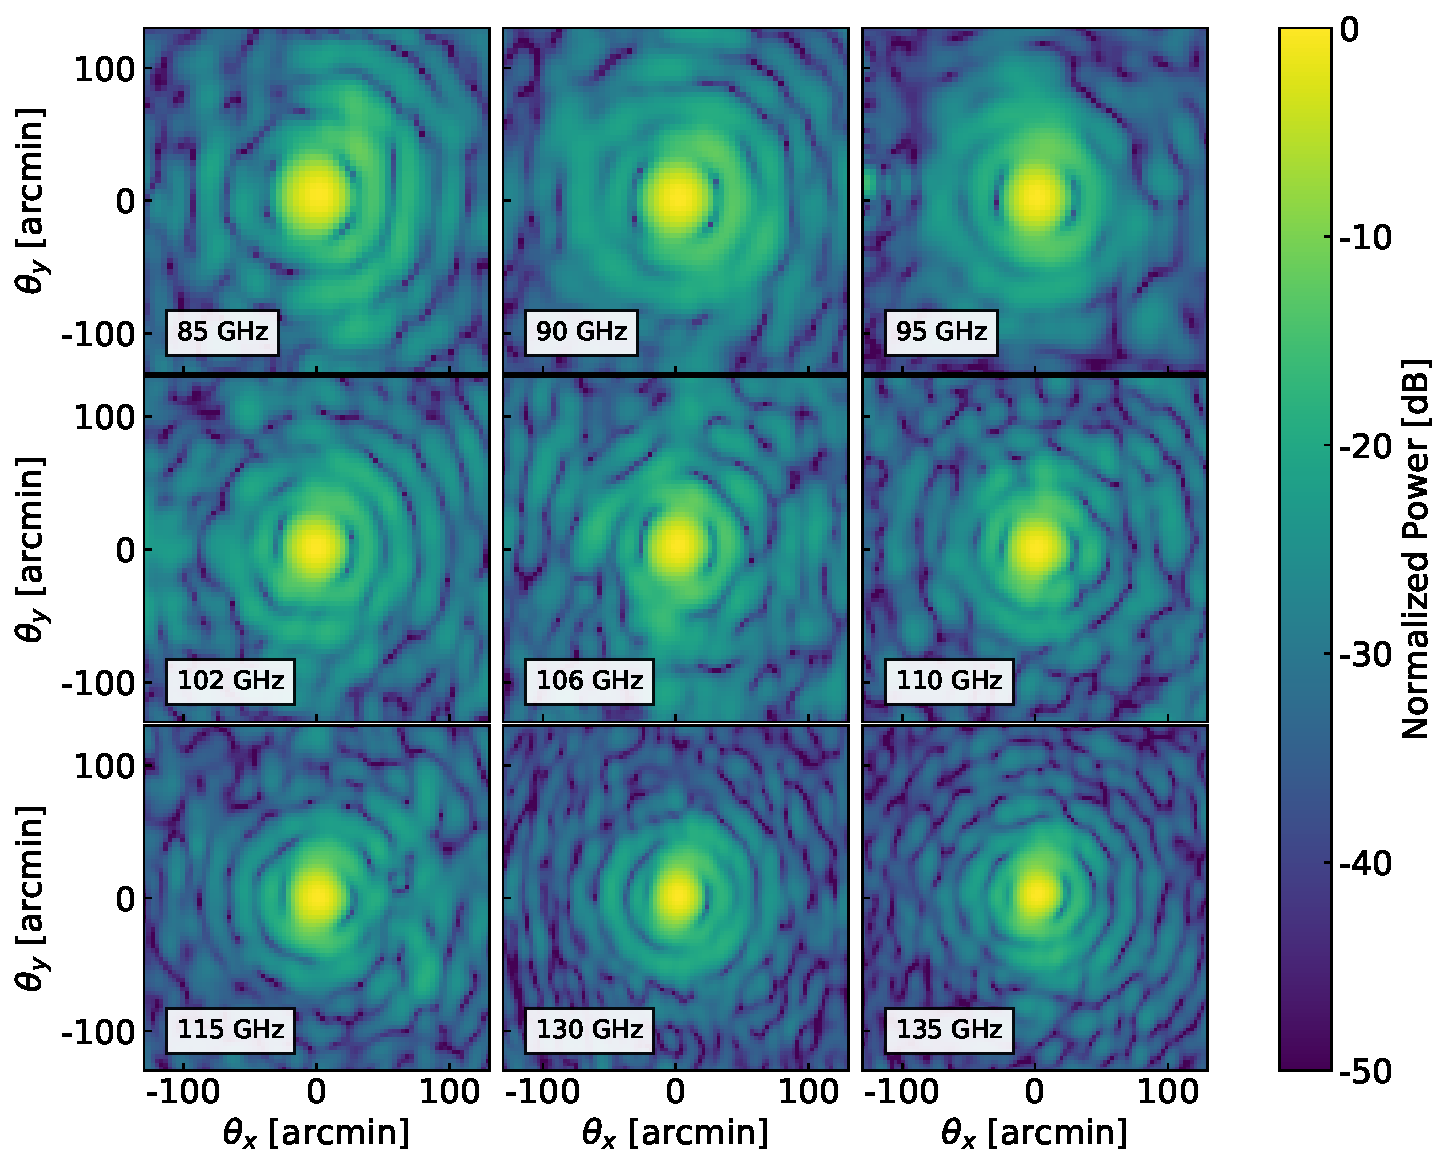
\includegraphics[width = \textwidth]{Figures/farfield_sat.pdf}
    \caption{Preliminary far-fields of the SAT optics tube in the MF-1.  The near-field measured beam is propagated to the far-field for each frequency.  The aliasing of the measured phase in the near-field (discussed in Section~\ref{sec:sat_results}) caused an artificial directional shift in the on-sky beam, which we center before plotting.}
    \label{fig:farfields_sat}
\end{figure*}

\subsection{Propagation of Fields}
\label{sec:sat_prop_fields}

The performance of the SAT optical system is assessed in detail by using the amplitude and phase of the measured beams to calculate the far-field.  This is carried out by using the Fourier relationship between the near-field $E(x,y)$ and far-field $B(\theta_x,\theta_y)$ beams \cite{McIntosh2016,alma_holog}:
\begin{equation}
    B(\theta_x,\theta_y) = \int_{\text{aperture}} E(x,y) e^{ i \frac{2\pi}{\lambda} (\theta_x x + \theta_y y )} dx \, dy 
\end{equation}
where the complex electric field $E(x,y)$ is integrated over the area of the aperture, $\theta_x$ and $\theta_y$ are the on-sky angular coordinates, and $\lambda$ is the wavelength.  

The resulting (preliminary) far-fields are shown in Figure~\ref{fig:farfields_sat}.  The measured beam size $26.02^{\prime}\pm YYY^{\prime}$ is consistent with the predicted F90 FWHM of $24.95^{\prime}$.

\section{Discussion}
\label{sec:sat_discussion}

We have presented holography measurements of the SO SAT optics tube and analysis methods determining its optical performance.  We further provide an open-source package for simulating near-field holography measurements and propagating the measurements into the far-field using Fourier optics.  From these data, we characterize the optical performance of the SAT MF optics tube.  We compare near- and far-field measurements to simulations.  After propagating the beams to the far-field, we find the SAT beam FWHM to be ($26.02^{\prime}\pm YYY^{\prime}$) in the F90 band, within the expected beam size of $24.95^{\prime}$, and is sufficient to accomplish SO's science goals at these angular scales.

We also provide \verb|sosat-optics|, an open-source software package, which models the SAT holography measurements and is customizable to include arbitrary optics and adaptable for other optics experiments~\cite{sat_sim_model}.  The approach demonstrated here follows the successful characterization of the Large Aperture Telescope Receiver tester, and is broadly applicable to other millimeter-wave optical systems~\cite{chesmore2022}.  The ability to characterize the optical performance and systematics of the optics tube allowed us to determine the SAT optics is in focus and that the beam is within requirement for SO science. 

\begin{figure}
    \centering
    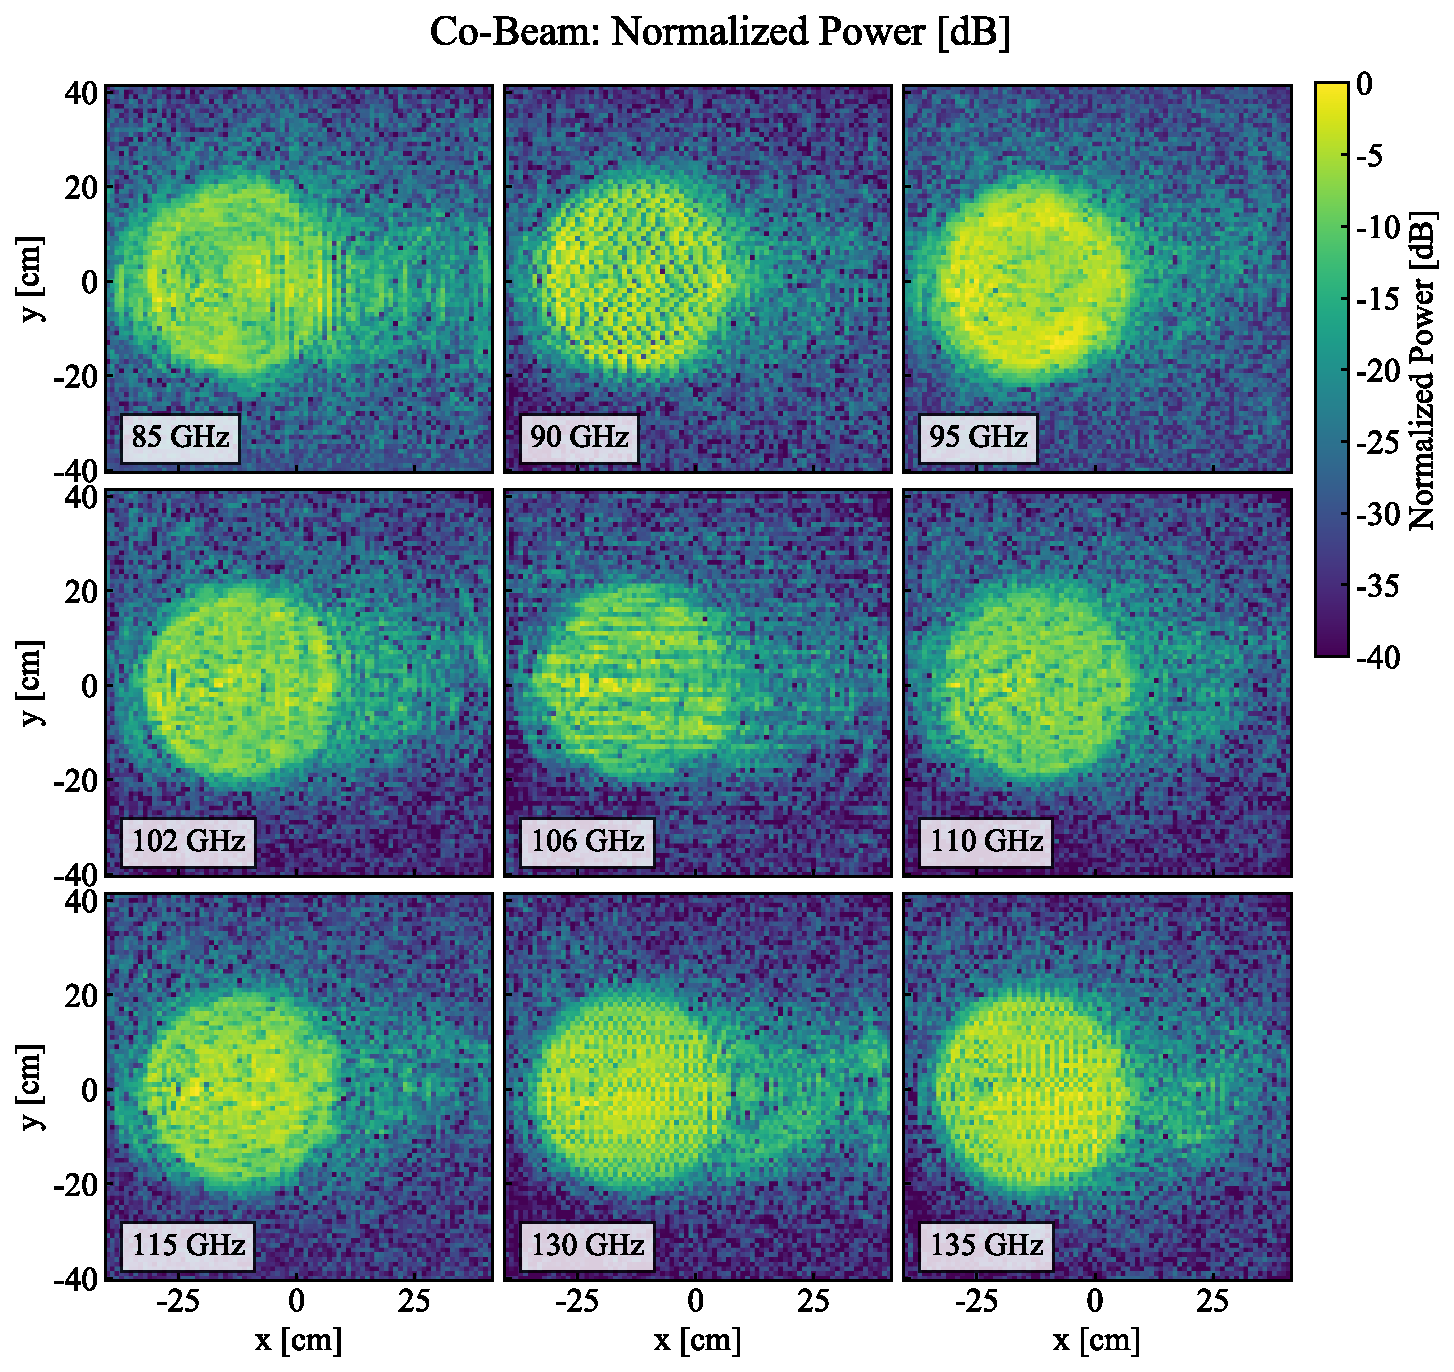
\includegraphics[width = \textwidth]{Figures/SAT_MF1_co-beam.pdf}
    \caption{Co-polar normalized power of the Simons Observatory Small Aperture Telescope near-field beam.}
    \label{fig:sat_mf_cobeam}
\end{figure}

\begin{figure}
    \centering
    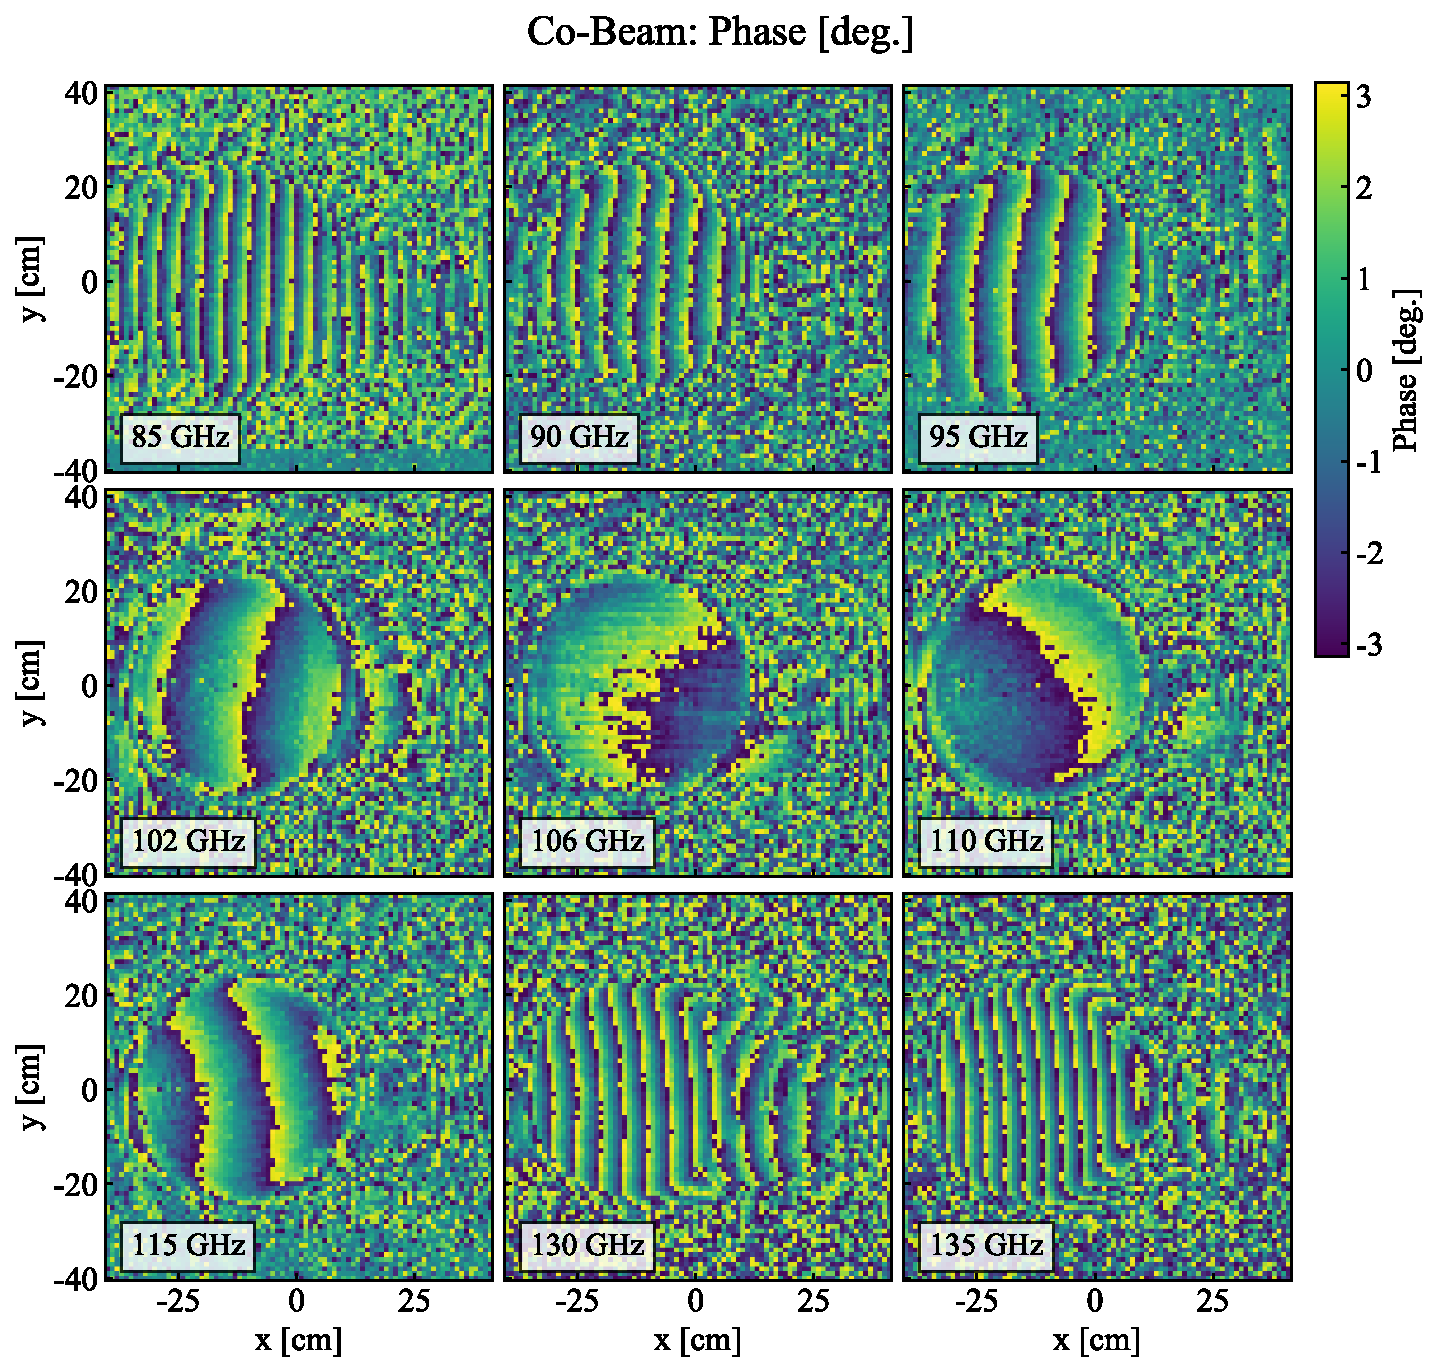
\includegraphics[width = \textwidth]{Figures/SAT_MF1_co-phase.pdf}
    \caption{Co-polar phase of the Simons Observatory Small Aperture Telescope near-field beam.}
    \label{fig:sat_mf_cophase}
\end{figure}

\begin{figure}
    \centering
    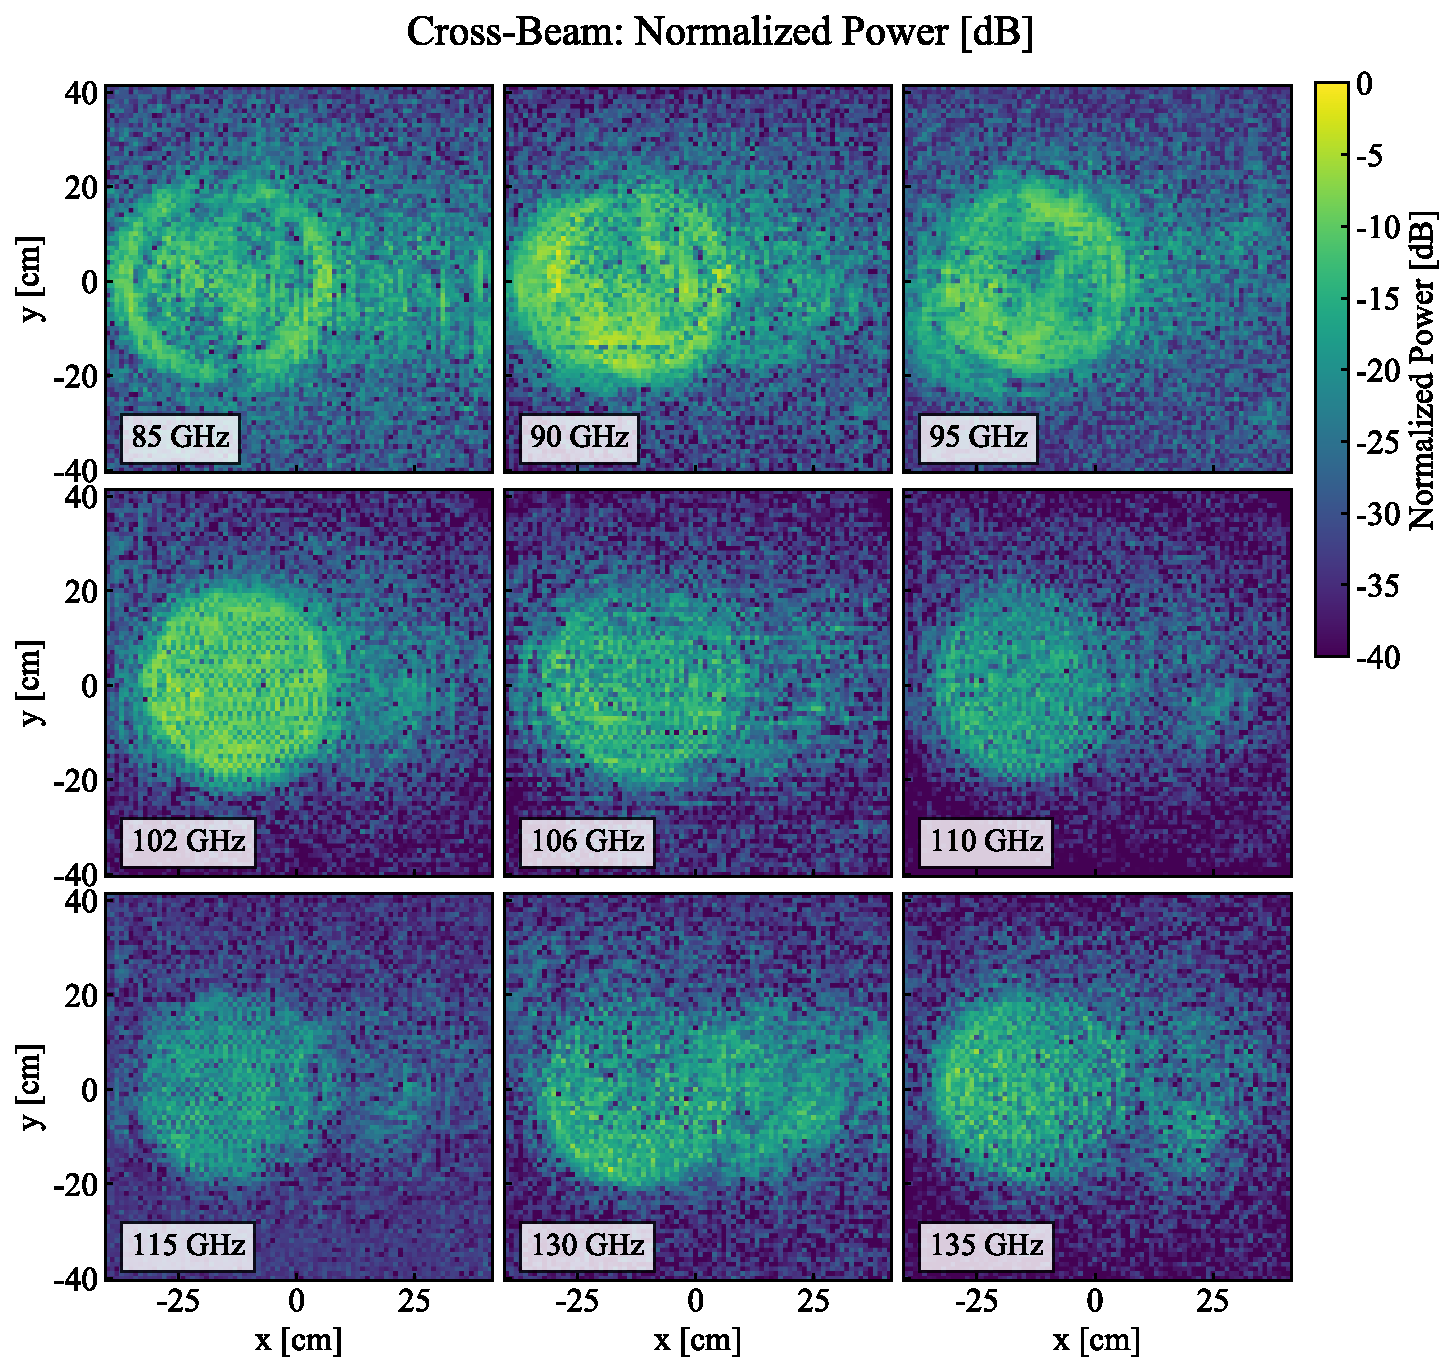
\includegraphics[width = \textwidth]{Figures/SAT_MF1_cr-beam.pdf}
    \caption{Cross-polar normalized power of the Simons Observatory Small Aperture Telescope near-field beam.}
    \label{fig:sat_mf_crbeam}
\end{figure}

\begin{figure}
    \centering
    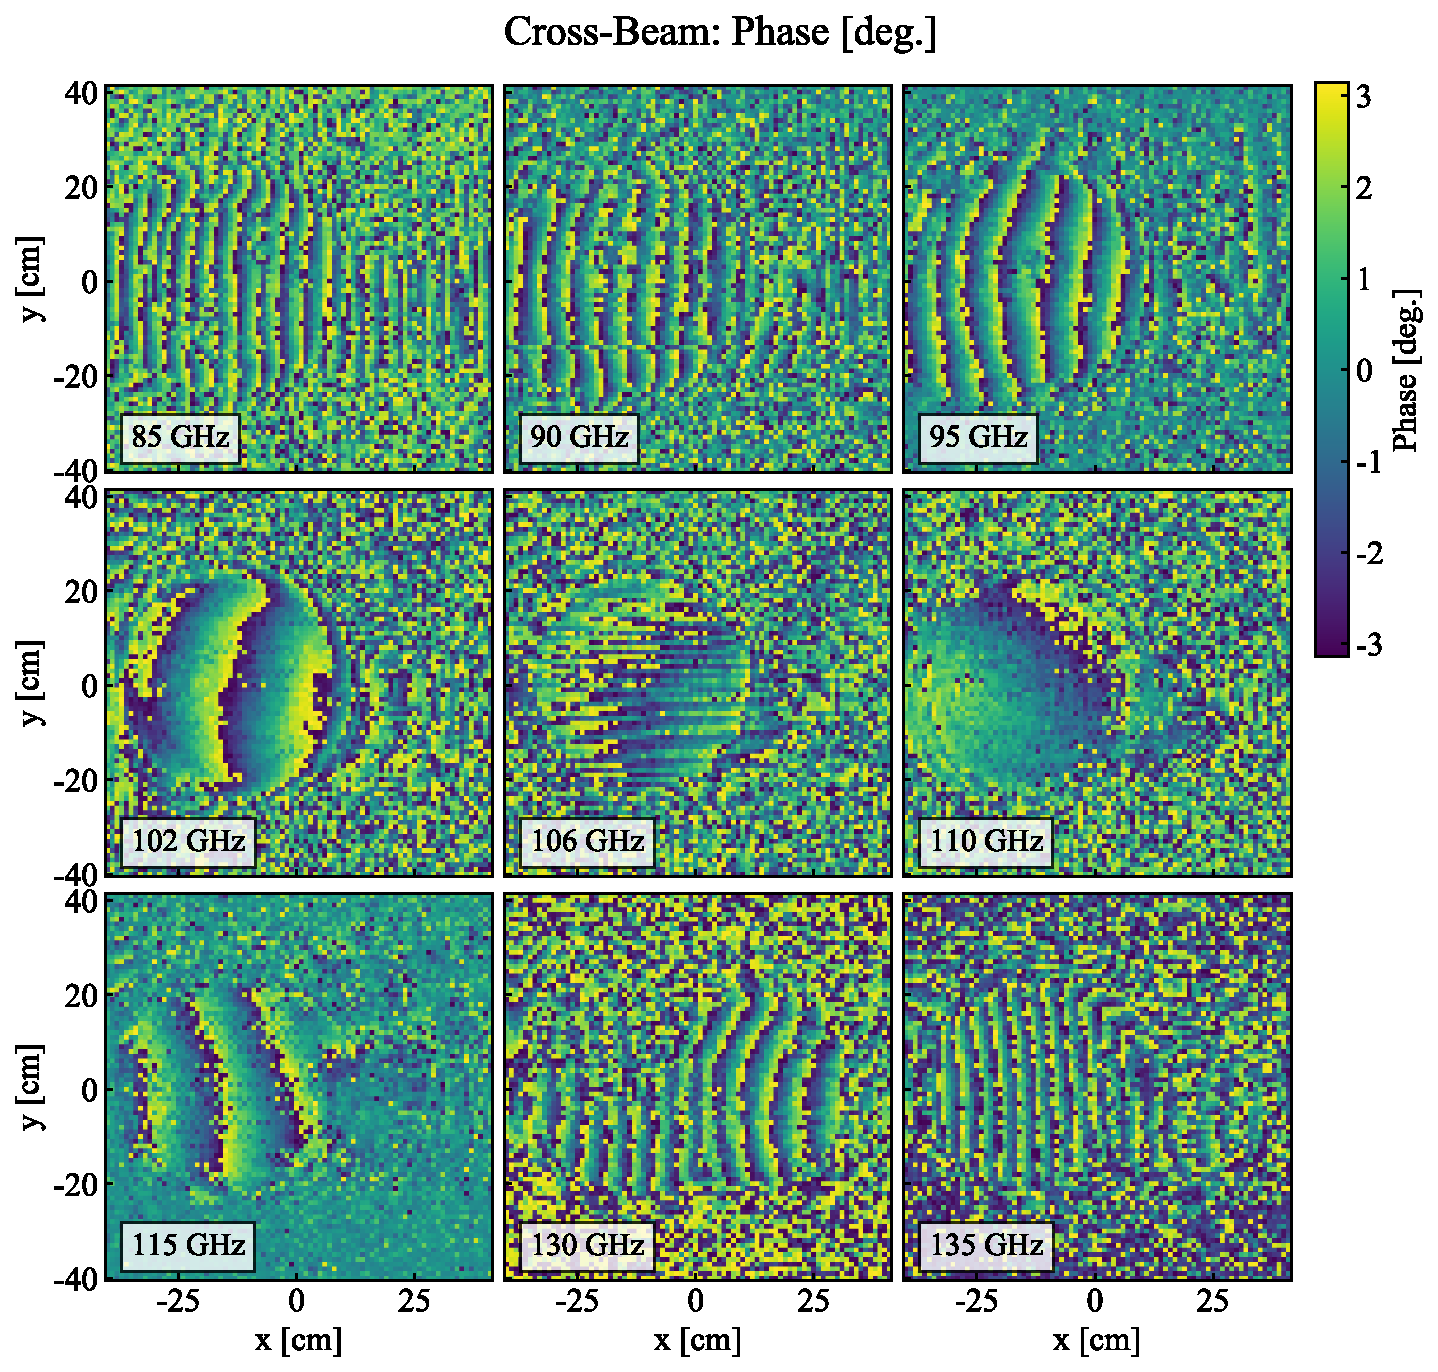
\includegraphics[width = \textwidth]{Figures/SAT_MF1_cr-phase.pdf}
    \caption{Cross-polar phase of the Simons Observatory Small Aperture Telescope near-field beam.}
    \label{fig:sat_mf_crphase}
\end{figure}
